\chapter{CNN Compiling in FPGAs}
\label{chapter:CNNVersat}

This chapter presents an overview of toolflows that map convolutional neural
networks into FPGA using the frameworks presented in
Section~\ref{section:darknet}. Next, the concepts for mapping CNNs
into CGRAs are introduced.

%PAPERS
%https://www.cv-foundation.org/openaccess/content_cvpr_workshops_2014/W17/html/Gokhale_A_240_G-opss_2014_CVPR_paper.html
%

\section{Toolflows for Mapping CNNs in FPGAs}
\label{section:toolflow}

Several software frameworks have been developed to accelerate development and
execution of CNNs. The neural networks frameworks discussed in
section~\ref{section:darknet} provide high level APIs together with high
performance execution on multi-core CPUs, GPUs, Digital Signal Processors (DSPs)
and Neural Processing Units (NPUs)~\cite{smartphones}. FPGAs provide an
alternative to these architectures as they provide high-performance while also
being low-power. FPGAs can meet several requirements like throughput and latency
in diversity of applications. Thus, several toolflows that map CNN descriptions
into hardware in order to perform inference have been created. In
table~\ref{table:toolflow}, a list of notable ones is presented.
\begin{table}[!htpb]
    \centering
    \begin{tabular}{lll}
    \hline
    \textbf{Toolflow Name} & \textbf{Interface}       & \textbf{Year}  \\ \hline
    fpgaConvNet            & Caffe \& Torch           & May 2016       \\
    DeepBurning            & Caffe                    & June 2016      \\
    Angel-Eye              & Caffe                    & July 2016      \\
    ALAMO                  & Caffe                    & August 2016    \\
    Haddoc2                & Caffe                    & September 2016 \\
    DNNWeaver              & Caffe                    & October 2016   \\
    Caffeine               & Caffe                    & November 2016  \\
    AutoCodeGen            & Proprietary Input Format & December 2016  \\
    Finn                   & Theano                   & February 2017  \\
    FP-DNN                 & Tensorflow               & May 2017       \\
    Snowflake              & Torch                    & May 2017       \\
    SysArrayAccel          & C                        & June 2017      \\
    FFTCodeGen             & Proprietary Input Format & December 2017  \\ \hline
    \end{tabular}
    \label{table:toolflow}
    \caption{CNN to FPGA Toolflows, adapted from~\cite{misc:cnntofpga}}
\end{table}


\subsection{Supported Neural Network Models}

These toolflows support the most common layers in CNNs, which are discussed in
chapter~\ref{chapter:cnn}. The acceleration target changes depending on the
toolflow.  For example, the fpgaConvNet~\cite{fpgaconvnet} toolflow focuses more
on feature extraction while offering non accelerated support for fully connected
layers.

\subsection{Architecture \& Portability}

\begin{figure}[!htbp]
    \centering
    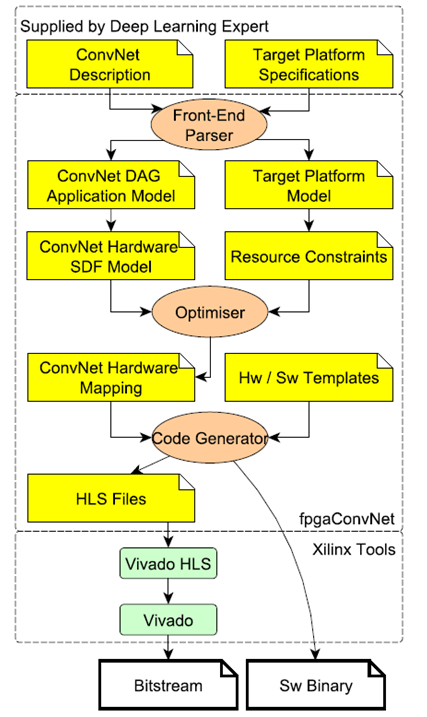
\includegraphics[width=0.5\textwidth]{Figures/fpgaconvnet.png}
    \caption{fpgaConvNet Architecture. Taken from~\cite{fpgaconvnet}}
    \label{figure:fpgaconvnet}
\end{figure}

As shown in figure~\ref{figure:fpgaconvnet}, the fpgaConvNet architecture
consists of a Front-End Parser that reads a (ConvNet) description of the network
and a description of the target platform and produces, on the one hand a
Directed Acyclic Graph (DAG), which is then converted to a Synchronous Data Flow
(SDF) hardware model, and on the other hand, a model of the target platform from
which resource constraints are derived. The hardware model thus obtained goes
into an Optimiser procedure, which produces a hardware mapping. Using hardware
and software templates, a Code Generator procedure, generates both the High
Level Synthesis (HLS) input files and the software binaries that will run on the
control CPU embedded in the FPGA. The HLS files go into the Xilinx (FPGA
manufacturer) tools so that the configuration bitstream of the FPGA is produced.

%\newpage
%\section{Optimizing Convolutional Layers}
%\label{section:autotuning}

%To perform Convolutional Layers, the most used algorithm is General Matrix Multiply (GEMM). First the input is converted with a step called
%im2col which transforms the 2D convolution into a Matrix Multiply.

%In Deep Versat,discussed in~\ref{chapter:DeepVersat}, due to the use of the Address Generating Units that can do 2 nested Loops, a single Versat Core
%can do a convolution on it's own


